\chapter{Valutazione dell'algoritmo}
In questo capitolo esamineremo la bontà dell'algoritmo implementato, 
confrontandolo con l'implementazione della funzione svd() presente nella 
libreria standard di MATLAB.

Verranno eseguiti i seguenti tipi di test:

\begin{enumerate}
	\item Test di accuratezza e misurazione dei tempi di calcolo su matrici $A$ 
ortogonali (matrici con condizionamento unitario);
	
	\item Test di accuratezza e misurazione dei tempi di calcolo su matrici 
malcondizionate (matrici di Hilbert e di Pascal);
	
	\item Test di accuratezza sul calcolo dei valori singolari, al variare del 
condizionamento della matrice di partenza.
\end{enumerate}

I test (assieme alla generazione dei grafici associati) sono stati implementati 
nello script 
\href{https://github.com/Yagotzirck/svd_benchmark/blob/main/src/benchmark_svd.m}{benchmark\_svd.m}, 
assieme alla classe 
\href{https://github.com/Yagotzirck/svd_benchmark/blob/main/src/BenchmarkSVD.m}{BenchmarkSVD.m} 
come supporto per l'esecuzione delle fattorizzazioni SVD e misurazione dei 
parametri relativi all'accuratezza e tempi di esecuzione.

\newpage
\section{Test su matrici ortogonali}
Iniziamo presentando il caso numericamente più stabile con matrici di partenza 
ortogonali $A \in \mathbb{R}^{n \times n}$, con $n$ nell'intervallo $[50, 800]$ 
ed uno step di 50 da una matrice all'altra.

La misura della precisione è basata sul fatto che in linea teorica, i vettori 
singolari dovrebbero essere ortonormali tra di loro, il che implica che
\begin{gather*}
	U^T U = I \\
	V^T V = I
\end{gather*}

Una stima dell'errore può essere quindi ricavata da
\begin{gather*}
	\| \mathbf{U^T U - I} \|_\infty \\
	\| \mathbf{V^T V - I} \|_\infty
\end{gather*}

I risultati sono stati i seguenti:

\begin{figure}[!htb]
\minipage{0.32\textwidth}
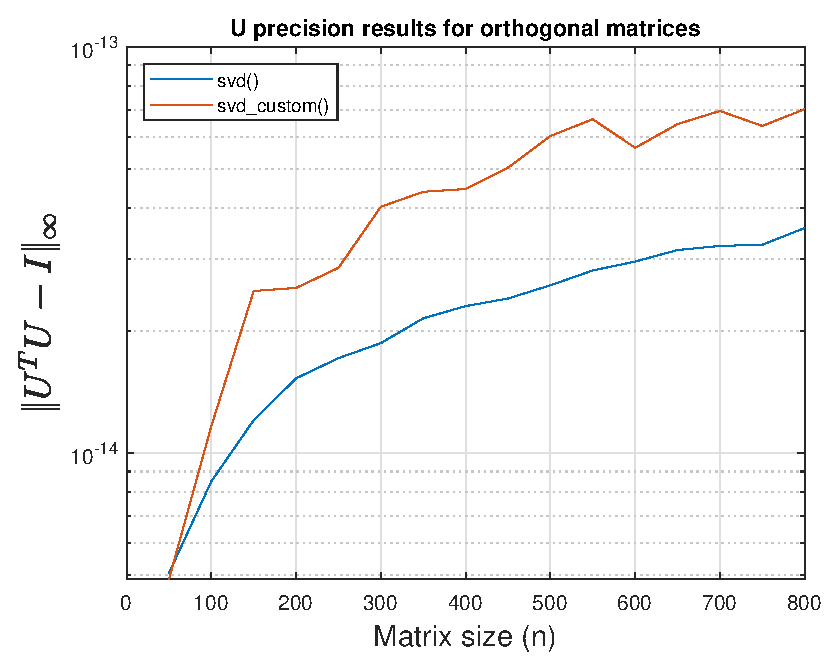
\includegraphics[width=\linewidth]{imgs/01_-_U_precision_results_for_orthogonal_matrices.eps}
\endminipage\hfill
\minipage{0.32\textwidth}  
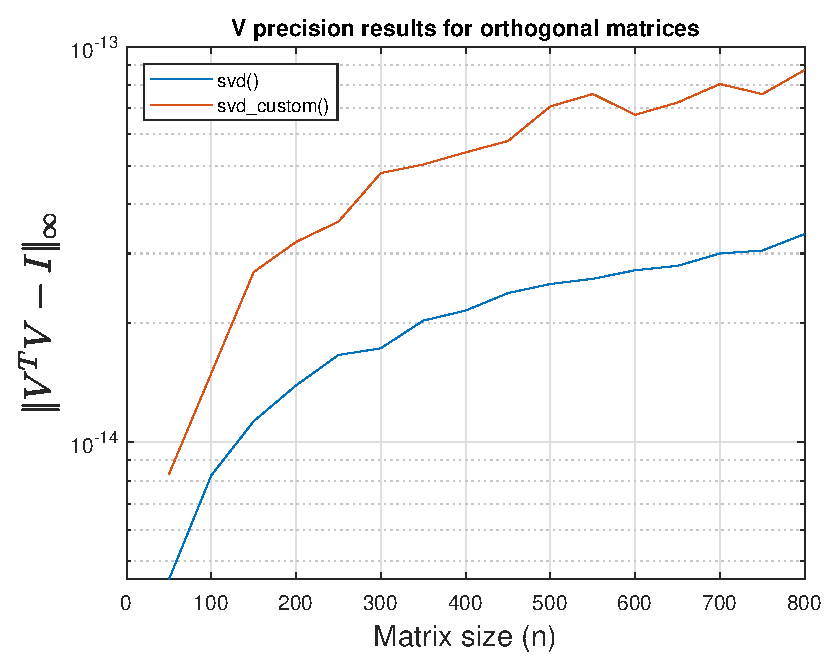
\includegraphics[width=\linewidth]{imgs/02_-_V_precision_results_for_orthogonal_matrices.eps}
\endminipage\hfill
\minipage{0.32\textwidth}  
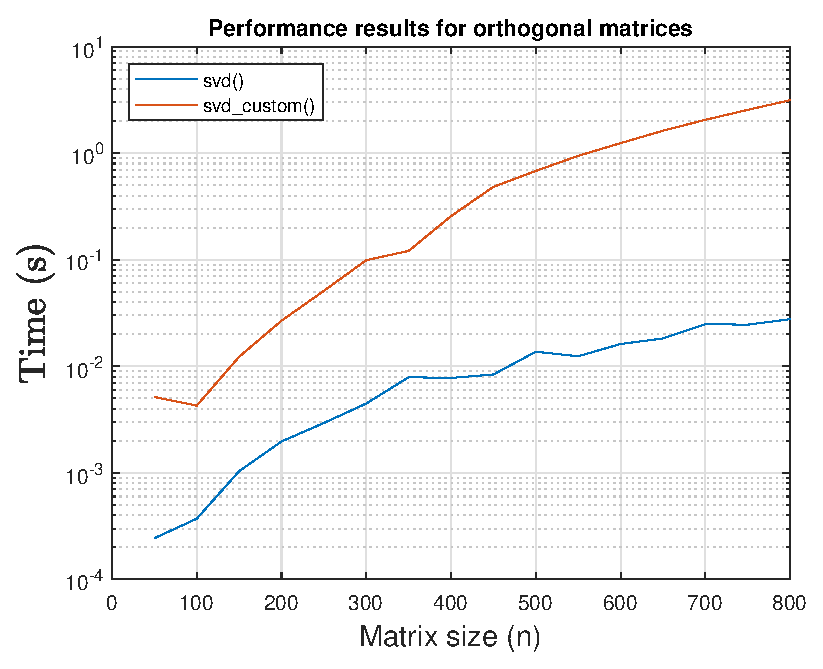
\includegraphics[width=\linewidth]{imgs/03_-_Performance_results_for_orthogonal_matrices.eps}
\endminipage
\end{figure}

Possiamo osservare come \textit{svd\_custom()} abbia precisione leggermente 
inferiore rispetto a \textit{svd()}, ma con risultati comunque molto buoni, con 
un errore che si tiene al di sotto di $10^{-13}$ per tutte le matrici $U,V$, 
anche con $n$ relativamente grande.

Per quanto riguarda i tempi di esecuzione, \textit{svd\_custom()} termina in un 
tempo che si aggira tra uno e due ordini di grandezza superiore rispetto a 
\textit{svd()} (3.13 secondi contro 0.03 secondi, per $n = 800$); nonostante non 
si tratti di un confronto alla pari dal momento che \textit{svd()} è una 
funzione compilata nativamente e non implementata come script MATLAB, il 
risultato ci fornisce comunque una stima sull'intrinseca inefficienza della 
fattorizzazione SVD ottenuta tramite il metodo degli autovalori di
$A^T A$ / $A A^T$, nonostante tutte le ottimizzazioni apportate.


\newpage
\section{Test su matrici malcondizionate}
Mostreremo ora la stessa tipologia di test mostrati nella sezione precedente, ma 
stavolta le matrici di partenza $A \in \mathbb{R}^{n \times n}$ sono due matrici 
malcondizionate:
\begin{itemize}
	\item Matrice di Hilbert;
	\item Matrice di Pascal.
\end{itemize}

Faremo variare $n$ all'interno di un intervallo più piccolo del precedente ($[2, 
100]$), con uno step unitario tra una matrice e la successiva.

\subsection{Matrice di Hilbert}

\begin{figure}[!htb]
\minipage{0.32\textwidth}
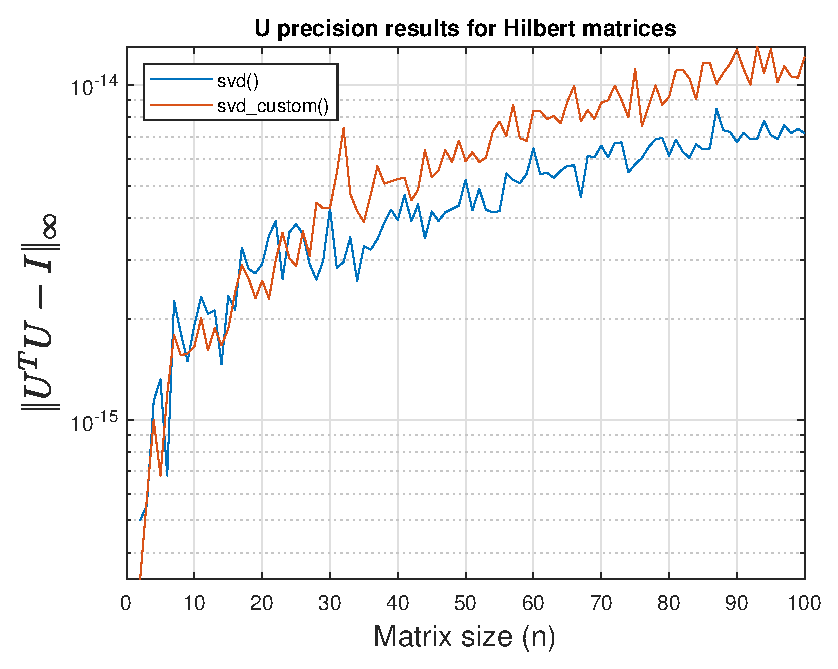
\includegraphics[width=\linewidth]{imgs/04_-_U_precision_results_for_Hilbert_matrices.eps}
\endminipage\hfill
\minipage{0.32\textwidth}  
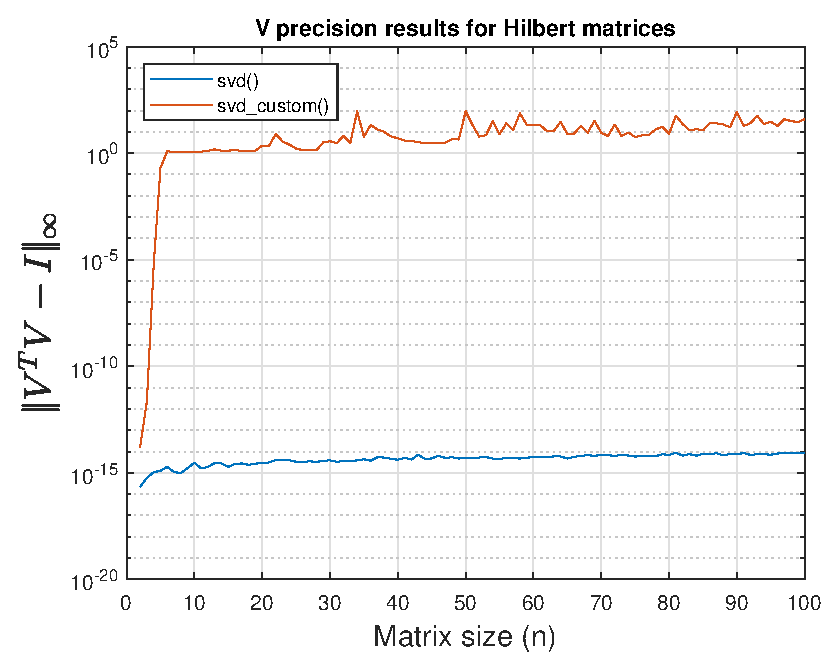
\includegraphics[width=\linewidth]{imgs/05_-_V_precision_results_for_Hilbert_matrices.eps}
\endminipage\hfill
\minipage{0.32\textwidth}  
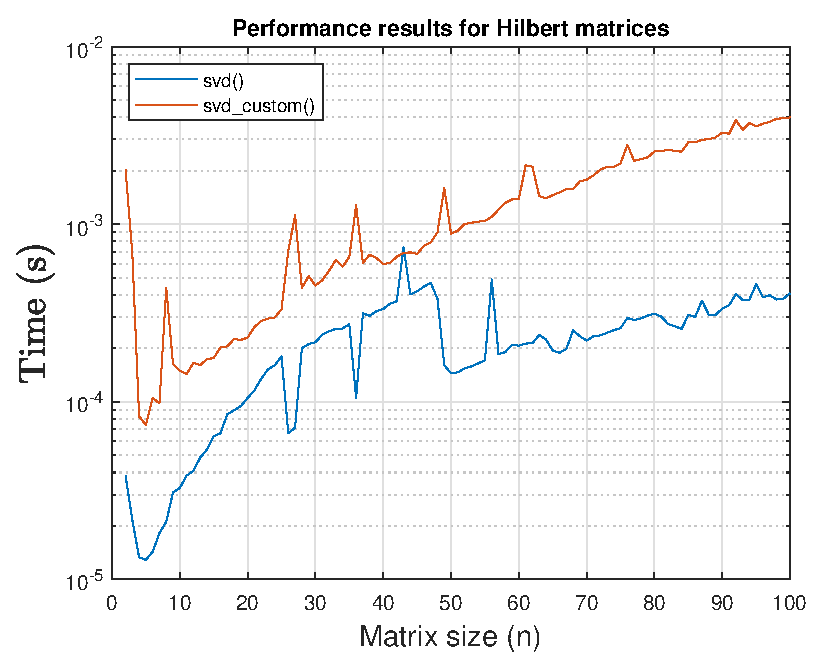
\includegraphics[width=\linewidth]{imgs/06_-_Performance_results_for_Hilbert_matrices.eps}
\endminipage
\end{figure}

In questo caso, la precisione di $U$ (derivata dall'algoritmo QR) continua ad 
essere più che buona, mentre $V$ (calcolata come $V = A^T U \Sigma_{k}^{-1}$) 
risente pesantemente del malcondizionamento di $A$, arrivando ad avere un errore 
unitario già a partire da $n = 6$ (che è un errore considerevole, in quanto 
significa che l'ortonormalità tra i vettori colonna di $V$ è stata completamente 
persa).

Non si notano invece differenze sostanziali nei tempi di calcolo rispetto ai 
test svolti sulle matrici ortogonali (i tempi per $n = 100$ risultano essere 
pressochè identici in entrambi i casi).


\newpage
\subsection{Matrice di Pascal}

\begin{figure}[!htb]
\minipage{0.32\textwidth}
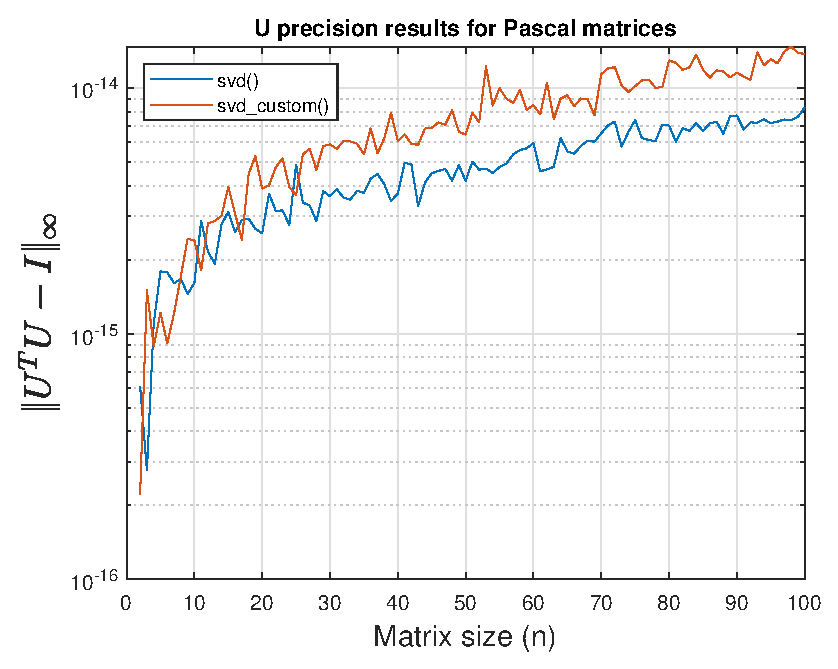
\includegraphics[width=\linewidth]{imgs/07_-_U_precision_results_for_Pascal_matrices.eps}
\endminipage\hfill
\minipage{0.32\textwidth}  
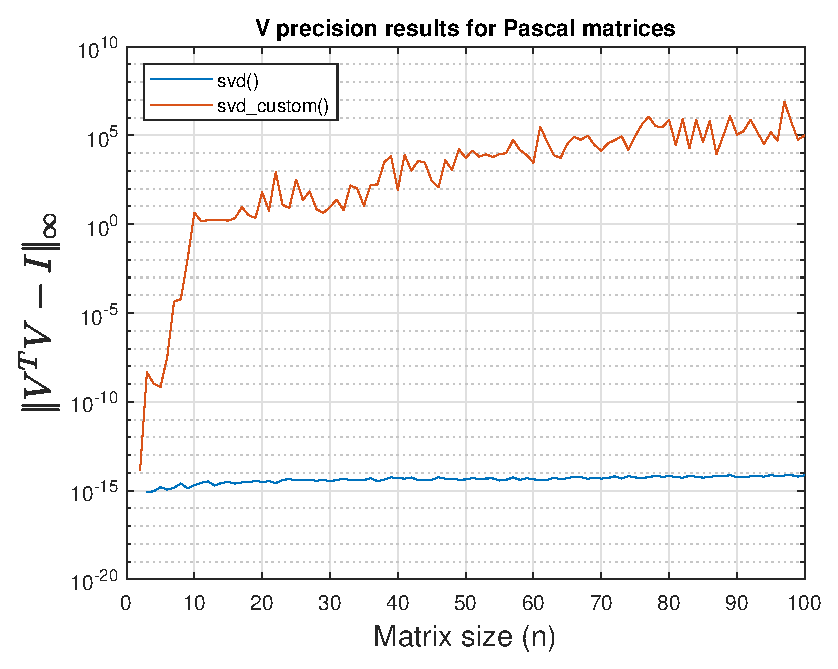
\includegraphics[width=\linewidth]{imgs/08_-_V_precision_results_for_Pascal_matrices.eps}
\endminipage\hfill
\minipage{0.32\textwidth}  
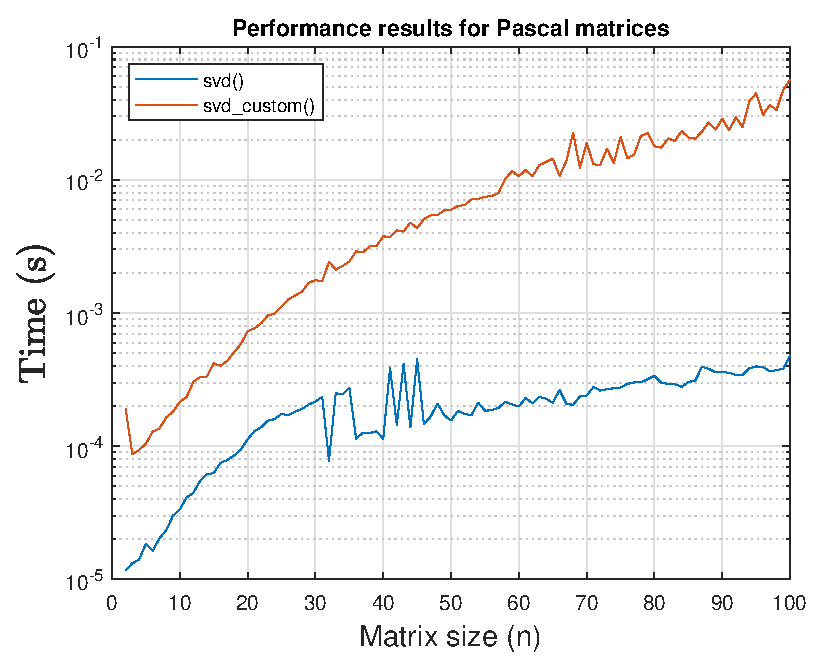
\includegraphics[width=\linewidth]{imgs/09_-_Performance_results_for_Pascal_matrices.eps}
\endminipage
\end{figure}

Possiamo osservare uno schema molto simile a quello riscontrato nella matrice di 
Hilbert, ma con gli errori in $V$ che presentano valori più alti.

Ciò è dovuto al fatto che gli errori in $V$ per la matrice di Hilbert sono 
quantitativamente mitigati dal fatto che
\begin{equation*}
	\lim_{n \to \infty} \max(hilb(n)(:)) = 1
\end{equation*}

Mentre per la matrice di Pascal si ha che
\begin{equation*}
	\lim_{n \to \infty} \max(pascal(n)(:)) = +\infty
\end{equation*}

In altri termini, i valori singolari della matrice di Hilbert tendono ad andare 
in \textbf{underflow}; viceversa, i valori singolari della matrice di Pascal 
tendono ad andare in \textbf{overflow}.


Tuttavia, al di là dell'errore quantitativo, in entrambi i casi i vettori della 
matrice $V$ perdono completamente la loro ortonormalità.

Inoltre, rispetto ai tempi osservati per la matrice di Hilbert, i tempi di 
calcolo per \textit{svd\_custom()} risultano essere di un ordine di grandezza 
più alti, mentre per \textit{svd()} si mantengono relativamente stabili.

\newpage
\section{Errori relativi sui valori singolari}
In questo tipo di test seguiremo un approccio differente: effettueremo 4 test, 
in cui verrà usata una matrice $A \in \mathbb{R}^{17 \times 17}$ costruita a 
partire da due matrici ortogonali $U, V$ ed una matrice $\Sigma_k$ contenente 17 
valori singolari noti, fissati in maniera tale che i numeri di condizionamento 
in norma 2 di $A$ siano i seguenti per ogni test:

\begin{center}
\begin{tabular}{|c|c|}
    \hline
    1. $\kappa_2(A) = 10^2$ & 2. $\kappa_2(A) = 10^4$ \\
    \hline
    3. $\kappa_2(A) = 10^8$ & 4. $\kappa_2(A) = 10^{16}$ \\
    \hline
\end{tabular}
\end{center}

Per ogni matrice costruiremo quindi un grafico avente sull'asse delle ascisse i 
valori singolari esatti $\sigma_i$, e sull'asse delle ordinate l'errore relativo 
del valore $\hat{\sigma}_i$ ottenuto dalle due funzioni \textit{svd()} e 
\textit{svd\_custom()}, calcolato come
\begin{equation*}
	\left\| \frac{\sigma_i - \hat{\sigma}_i}{\sigma_i} \right\|
\end{equation*}

I risultati sono stati i seguenti:

\begin{figure}[!htb]
\minipage{0.45\textwidth}
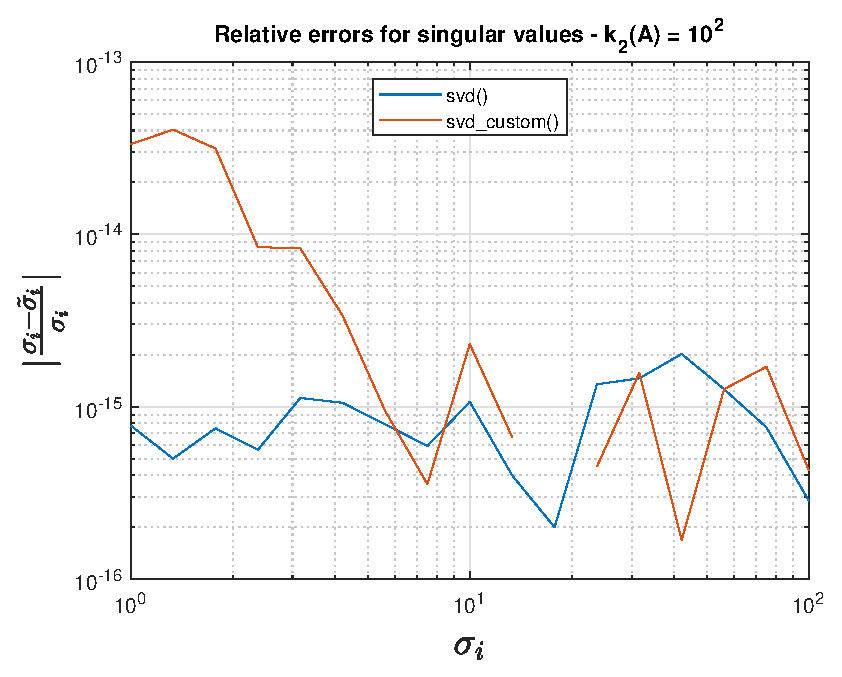
\includegraphics[width=\textwidth]{imgs/10_-_Relative_errors_for_singular_values_-_k_2(A)_=_10^2.eps}
\endminipage\hfill
\minipage{0.45\textwidth}  
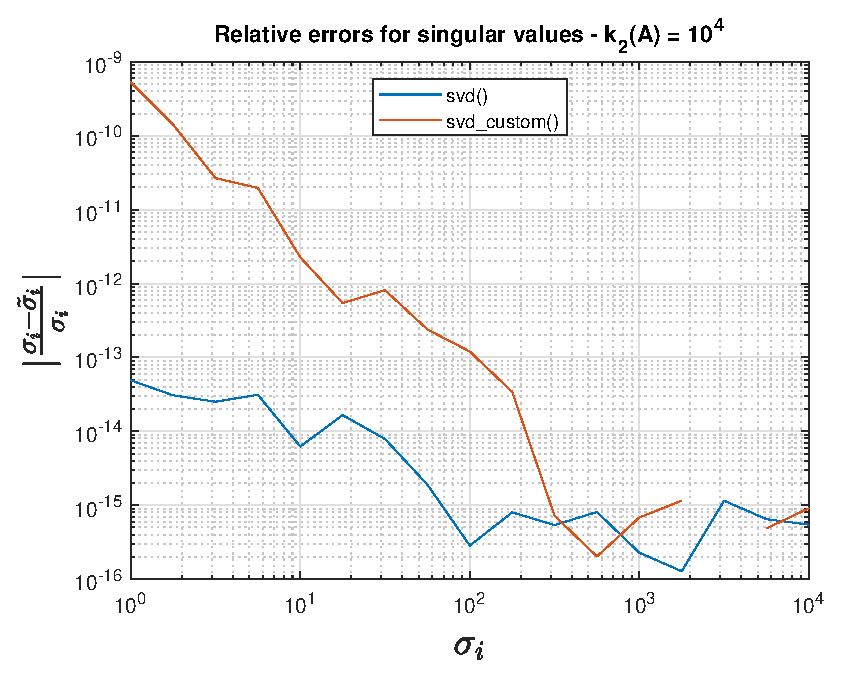
\includegraphics[width=\textwidth]{imgs/11_-_Relative_errors_for_singular_values_-_k_2(A)_=_10^4.eps}
\endminipage
\end{figure}


\begin{figure}[!htb]
\minipage{0.45\textwidth}
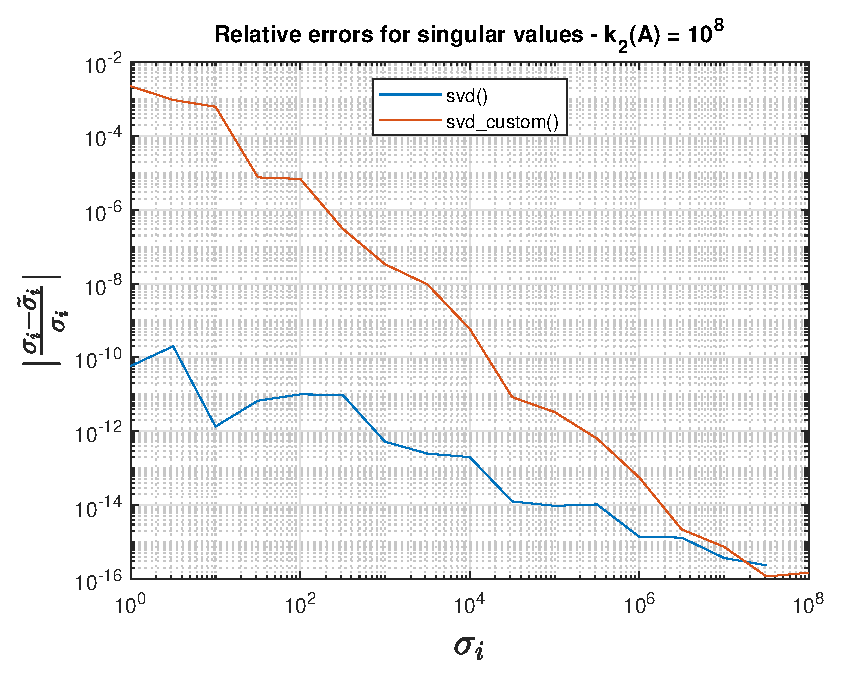
\includegraphics[width=\textwidth]{imgs/12_-_Relative_errors_for_singular_values_-_k_2(A)_=_10^8.eps}
\endminipage\hfill
\minipage{0.45\textwidth}  
\includegraphics[width=\textwidth]{imgs/13_-_Relative_errors_for_singular_values_-_k_2(A)_=_10^{16}.eps}
\endminipage
\end{figure}

Le discontinuità riscontrate in alcuni punti sono dovute ad errori relativi 
esattamente uguali a 0, e lo 0 esatto non è rappresentabile nei grafici di 
MATLAB con scala logaritmica generati con la funzione \textit{loglog()}.

Ciò che possiamo osservare è che per entrambe le funzioni, il valore singolare 
più piccolo tende ad essere quello che risente maggiormente del condizionamento 
della matrice, fino ad arrivare al valore singolare più grande in cui l'errore 
relativo sembra invece annullarsi.

Inoltre, prendendo come riferimento il valore singolare più piccolo $\sigma_n$ 
ed il numero di condizionamento pari a $10^k$, possiamo osservare che
\begin{itemize}
\item Per \textit{svd()}, si ha che $\left\| \frac{\sigma_n - 
\hat{\sigma}_n}{\sigma_n} \right\| \approx 10^{16 - k}$;
\item Per \textit{svd\_custom()}, si ha che $\left\| \frac{\sigma_n - 
\hat{\sigma}_n}{\sigma_n} \right\| \approx 10^{16 - k^2}$
\end{itemize}

Ciò è dovuto al fatto che l'algoritmo implementato lavora su $B = A A^T$ (oppure 
su $B = A^T A$), e dal momento che $\kappa_2(B) = (\kappa_2(A))^2$, anche gli 
errori assoluti dei valori singolari calcolati saranno elevati al quadrato; 
mentre per valori singolari grandi l'errore relativo viene smorzato rispetto 
all'errore assoluto con la divisione al denominatore, con valori singolari 
piccoli tale smorzamento non avviene, portando ai risultati mostrati nei grafici 
sopra con errori relativi decrescenti al crescere di $\sigma_i$.



\section{Overflow e underflow}
\subsection{Overflow}
Posto il massimo valore rappresentabile in double precision
\begin{equation*}
	v_{max} \approx 10^{308}
\end{equation*}

L'algoritmo implementato va in overflow con matrici $A$ aventi valori singolari
\begin{equation*}
	\sigma_i \geq \sqrt[4]{v_{max}} \approx 10^{77}
\end{equation*}

Ciò è dovuto al fatto che
\begin{enumerate}
	\item Un primo "elevamento al quadrato" degli $a_{ij} \in A$ si ha calcolando 
$B = A A^T$ oppure $B = A^T A$;
	\item Un secondo "elevamento al quadrato" lo si ha nella tridiagonalizzazione 
di $B$, più precisamente nella costruzione della matrice di Householder per ogni 
colonna di $B$.
	
	Infatti, i passi per la costruzione della matrice sono:
	\begin{enumerate}
		\item $\sigma = \| x \|_2$
		\item $k = -\sgn(x) \cdot \sigma$
		\item $\beta = \sigma (\sigma + | x_1 |)$
		\item $v = x - k \cdot e_1$
		\item $H = I - \frac{1}{\beta}v v^T $
	\end{enumerate}
	
	Al passo (c) viene calcolato un \textbf{quadrato della norma di un vettore} di 
$B$, ed al passo (e) viene usato tale valore come divisore per gli elementi 
della matrice risultante da un \textbf{outer product} (altro "elevamento a 
quadrato" degli elementi di un vettore di $B$).
\end{enumerate}

Se $A$ possiede degli elementi $|a_{ij}| \geq \sqrt[4]{v_{max}}$ \textit{(e li 
ha quasi sicuramente, se possiede uno o più valori singolari $\sigma_i \geq 
\sqrt[4]{v_{max}}$)}, al passo (e) vengono effettuate delle divisioni 
$\frac{\infty}{\infty}$, che portano ad avere una matrice con valori 
\textit{NaN}.



\subsection{Underflow}
Con un procedimento del tutto analogo a quello presentato sopra per l'overflow, 
possiamo concludere che, posto il minimo valore positivo rappresentabile in 
double 
precision
\begin{equation*}
	v_{min} \approx 10^{-308}
\end{equation*}

L'algoritmo implementato va in underflow con matrici $A$ aventi valori singolari
\begin{equation*}
	\sigma_i \leq \sqrt[4]{v_{min}} \approx 10^{-77}
\end{equation*}

